\documentclass[tikz,border=2mm]{standalone}
\usepackage{tikz}
\usetikzlibrary{positioning}

\begin{document}
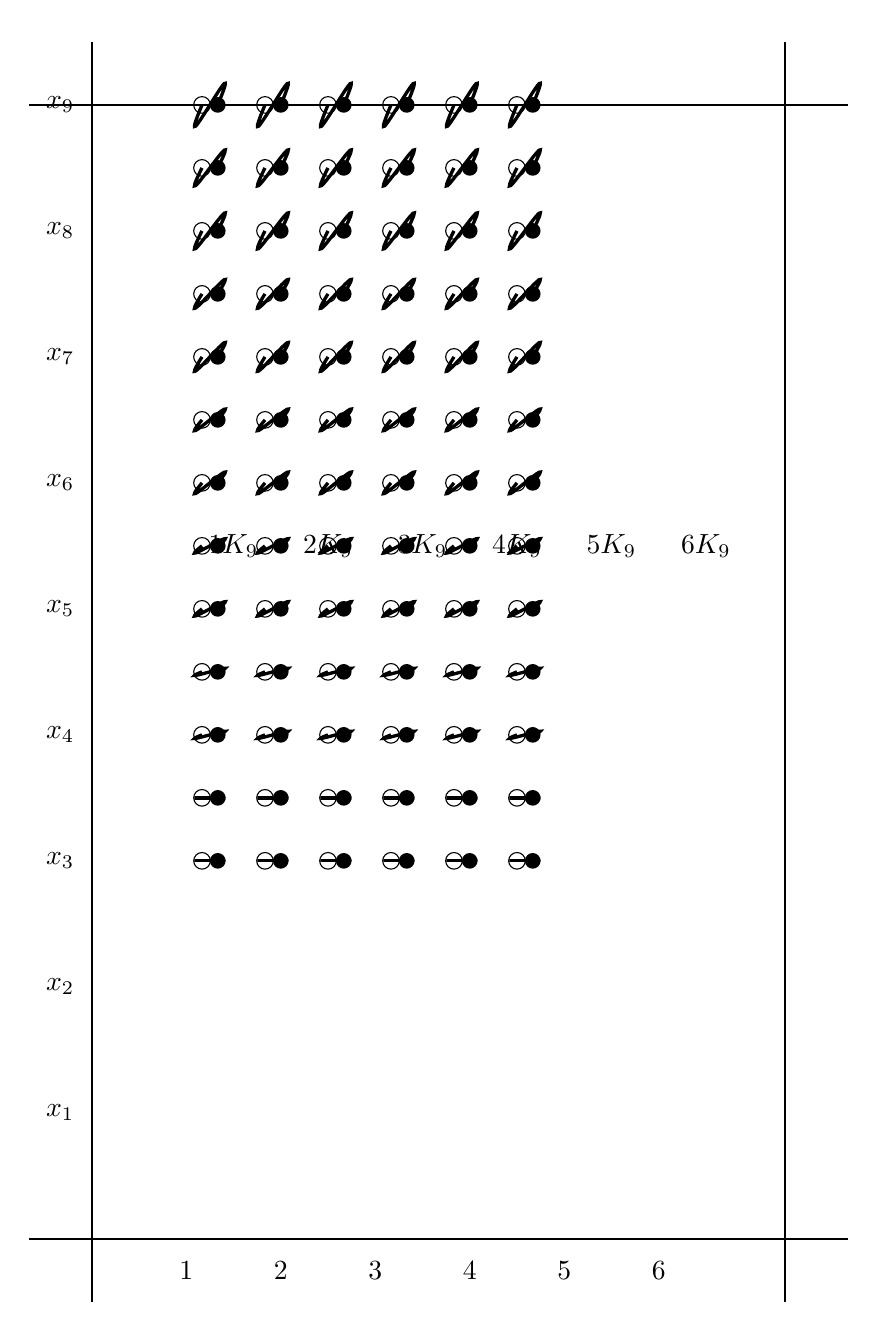
\begin{tikzpicture}[scale=0.8]

% Define node styles
\tikzset{
    dot/.style = {circle, fill, inner sep=2pt},
    circ/.style = {circle, draw, minimum size=6pt, inner sep=0pt},
}

% Draw vertical lines for x-axis labels
\draw [thick] (0,-13) -- (0,7);
\draw [thick] (11,-13) -- (11,7);

% Draw horizontal lines for separation
\draw [thick] (-1,-12) -- (12,-12);
\draw [thick] (-1,6) -- (12,6);

% Place x-axis labels
\node at (-0.5,6) {$x_9$};
\node at (-0.5,4) {$x_8$};
\node at (-0.5,2) {$x_7$};
\node at (-0.5,0) {$x_6$};
\node at (-0.5,-2) {$x_5$};
\node at (-0.5,-4) {$x_4$};
\node at (-0.5,-6) {$x_3$};
\node at (-0.5,-8) {$x_2$};
\node at (-0.5,-10) {$x_1$};

% Place x-axis numbers
\node at (1.5,-12.5) {1};
\node at (3,-12.5) {2};
\node at (4.5,-12.5) {3};
\node at (6,-12.5) {4};
\node at (7.5,-12.5) {5};
\node at (9,-12.5) {6};

% Place K_9 cluster labels
\node at (2.25,-1) {$1K_9$};
\node at (3.75,-1) {$2K_9$};
\node at (5.25,-1) {$3K_9$};
\node at (6.75,-1) {$4K_9$};
\node at (8.25,-1) {$5K_9$};
\node at (9.75,-1) {$6K_9$};

% Draw clusters of dots and circles
\foreach \i/\j in {2/1, 3/2, 4/3, 5/4, 6/5, 7/6}
{
    % Draw filled dots (black)
    \foreach \k in {-6,-5,...,6}
    {
        \node [dot] at (\i,\k) {};
    }
    
    % Draw unfilled circles (white)
    \foreach \k in {-6,-5,...,6}
    {
        \node [circ] at (\j+0.75,\k) {};
    }
    
    % Draw connecting curves
    \foreach \k in {-6,-5,...,6}
    {
        \pgfmathtruncatemacro{\shift}{(\k+6)/2}
        \draw [very thick] (\i,\k) .. controls ++(0.5,\shift*0.2) and ++(-0.5,-\shift*0.2) .. (\j+0.75,\k);
    }
}

\end{tikzpicture}
\end{document}